\documentclass[a4paper,12pt]{article}
\usepackage[utf8]{inputenc}
\usepackage[colorlinks=false,breaklinks=true]{hyperref}

\usepackage[british]{babel}

\usepackage{color}
\usepackage{ulem}
\usepackage{caption}
\usepackage{float}
\usepackage{subcaption}

\usepackage[dvips]{graphicx}

\usepackage{pstricks}
\usepackage{geometry}

\usepackage[onehalfspacing]{setspace}

\geometry{verbose,tmargin=1in,bmargin=1in,outer=1in, inner=1in}

\title{Behavioral Cloning Project}

\begin{document}

\maketitle

The goals of this project are the following:
\begin{itemize}
  \item Use the simulator to collect data of good driving behavior.
  \item Build a convolution neural network in Keras that predicts steering angles from images.
  \item Train and validate the model with the training and validation sets.
  \item Test that the model successfully drives around track one without leaving the road.
  \item Summarize the results with a written report.
\end{itemize}

I will consider the \href{https://review.udacity.com/#!/rubrics/432/view}{rubric points} individually and describe how I addressed each point in my implementation.  

\section{Required Files Submitted \& Code Quality}

The submission includes all required files that can be used to run the simulator in the autonomous mode:
\begin{itemize}
  \item \texttt{drive.py} for driving the car in autonomous mode;
  \item \texttt{model.h5} containing a trained convolution neural network;
  \item \texttt{model.py} containing the script to create and train the model;
  \item \texttt{video.mp4} containing a video with the car driving in autonomous mode;
  \item \texttt{writeup.pdf} summarizing the results.
\end{itemize}

\section{Code Quality}

\subsection{Functional Code}
Using the Udacity provided simulator and the \texttt{drive.py} file, the car can be driven autonomously around the track by executing
\begin{verbatim}
python drive.py model.h5
\end{verbatim}
with the speed up to 15 mph.

\subsection{Usable and readable code}
The \texttt{model.py} file contains the code for preparing data, training and saving the convolution neural network. The file shows the pipeline I used for training and validating the model. In addition, it contains self explanatory comments.

\section{Model Architecture and Training Strategy}

\subsection{An appropriate model architecture has been employed}
The data in my model is normalized using a Keras lambda layer (\texttt{model.py} line 115). My model consists of a convolution neural network with $5 \times 5$ and $3 \times 3$ filter sizes and depths between 24 and 64 (\texttt{model.py} lines 117-121). The model includes \textit{RELU} activation functions to introduce nonlinearity in each convolution layer (\texttt{model.py} lines 117-121). 

\subsection{Attempts to reduce over-fitting in the model}
The model is trained and validated on different data sets to ensure that the model was not over-fitting (\texttt{model.py} line 39). The training data set is represented by 80\% of the input data, whereas 20\% of the input data is associated with the validation data set. The model is tested by running it through the simulator and ensuring that the vehicle can stay on the track.

To reduce over-fitting, the model includes dropout layers between fully connected layers (\texttt{model.py} lines 124-129).

\subsection{Model parameter tuning}
The model uses an Adam optimizer (\texttt{model.py} line 132), therefore the learning rate is tuned automatically.

\subsection{Appropriate training data}
The training data is chosen to keep the vehicle driving on the road. To achieve this behavior, I use a combination of center lane driving, left and right lane driving (see the next section for details of the training data creation).

\section{Architecture and Training Documentation}

\subsection{Solution Design Approach}
To derive the correct model architecture, a number of steps was taken. I started with a neural network model with low complexity similar to \textit{LeNeT-5}. This model could already be trained in the way that the car was driving a part of the track autonomously. Of course, since the mean squared error was too high on the validation set, the steering angles were not always predicted correctly, and the car fell off the track.

My next step was to use data preprocessing to get better data input. In this step the data was normalized and cropped inside the neural network. This in turn made the mean squared error lower. I also used all three cameras provided by the simulator with adjusted steering angles to avoid the car driving off the track.

To improve the steering angle prediction, I used the model published by the autonomous vehicle team from \textit{Nvidia}. This model predicts the steering angles good enough, such that the vehicle is able to drive autonomously around the track without leaving the road.

I generalized training data by augmenting the collected images. Using a simplest augmentation technique, I added the flipped images with an inverted steering angle sign to the data set during the training process. Unfortunately, the training data set became too big to fit into the memory. Therefore, I included a generator function that split the data on batches. The size of batches equals to 32 such that the training data fits into the memory of my computer. In addition, to reduce the execution time, I installed the tensorflow library with GPU support and performed all operations on my Nvidia GPU. When fine-tuning the model, I configured an AWS instance with multiple GPUs and trained the model there.

At the end of the process, the vehicle was able to drive autonomously around the track without leaving the road in the both forward and backward direction (see \texttt{video.mp4}).

\subsection{Final Model Architecture}
The final model architecture is an extended version of the one presented by the \textit{Nvidia} autonomous vehicle team. In addition to the features of the \textit{Nvidia} model, my model includes the dropout layers between each fully connected layer to avoid over-fitting.

The first layer normalizes the input images mapping the RGB input from 0 to 255 to $-0.5$ to $0.5$ (\texttt{model.py} line 115). The second layer crops the input images cropping top 67 pixels and bottom 25 pixels (\texttt{model.py} line 116). The image size changes from (160, 320, 3) to (68, 320, 3). The next five convolutional layers use the \textit{RELU} activation function. The first 3 convolutional layers apply $5\times 5$ filters (\texttt{model.py} lines 117-119), whereas the last two apply $3 \times 3$ (\texttt{model.py} lines 120-121).

After flattering the model with the next layer (\texttt{model.py} line 123), the set of fully connected layers are added with a dropout with probability $0.2$ in between (\texttt{model.py} lines 124-130).

The visualization of the architecture is constructed using \textit{keras.utils.visualize\_util}:
\begin{figure}[H]
\centering
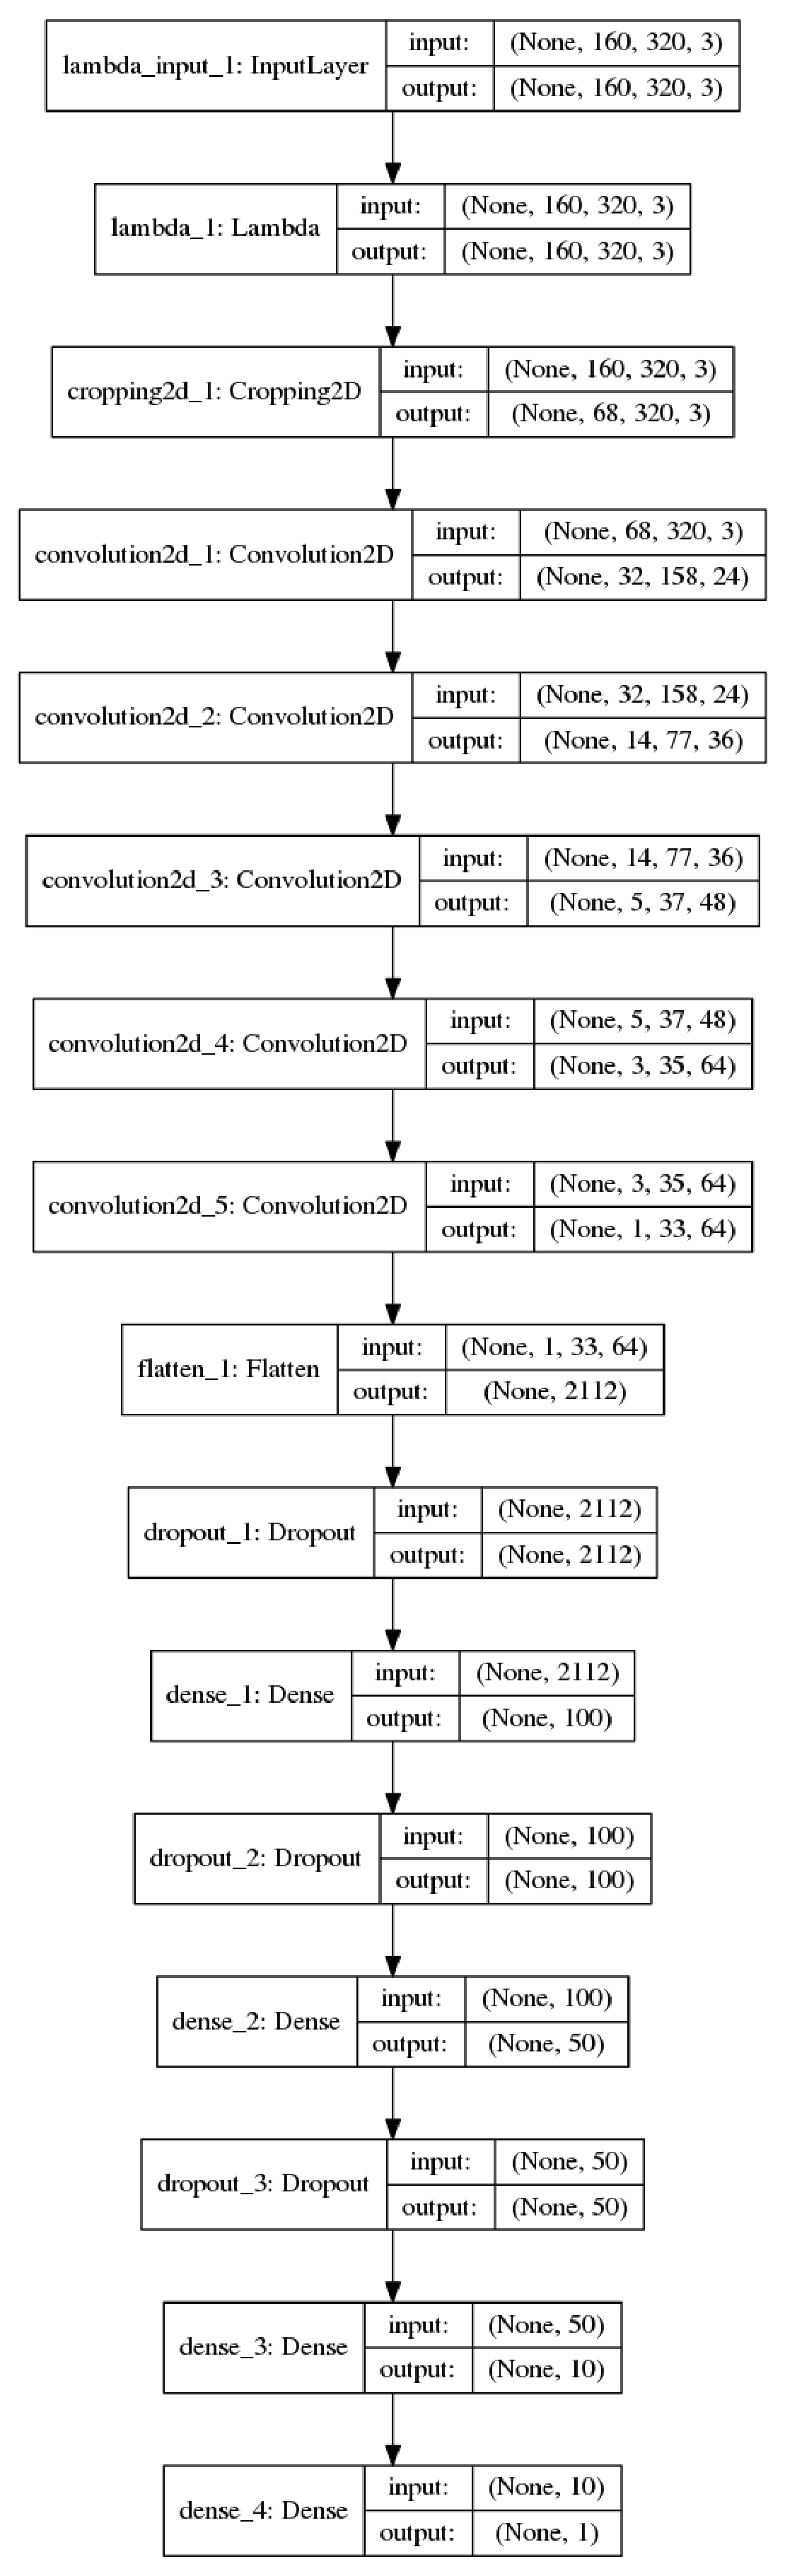
\includegraphics[height=22.5cm]{figures/model.eps}
\label{fig:effort}
\caption{Model architecture}
\end{figure}

\subsection{Creation of the Training Set \& Training Process}
To capture good driving behavior, I first recorded two laps on track one using center lane driving. Here is an example image of center lane driving:

\begin{figure}[H]
\centering
\begin{subfigure}{.3\textwidth}
  \centering
  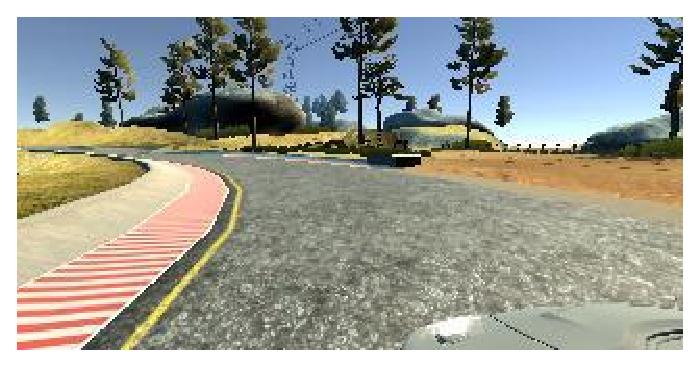
\includegraphics[width=0.98\linewidth]{figures/center_left.eps}
  \caption{Left camera}
\end{subfigure}
\begin{subfigure}{.3\textwidth}
  \centering
  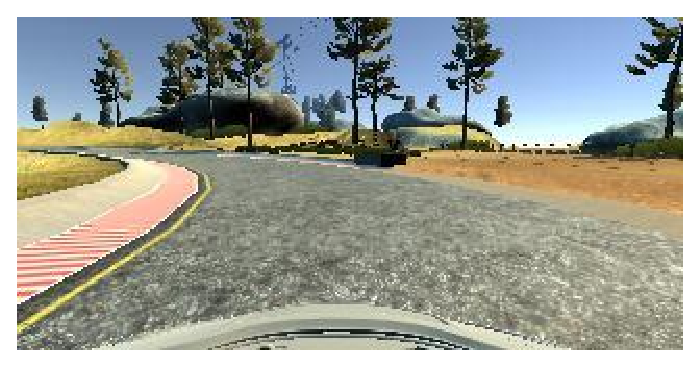
\includegraphics[width=0.98\linewidth]{figures/center_center.eps}
  \caption{Center camera}
\end{subfigure}
\begin{subfigure}{.3\textwidth}
  \centering
  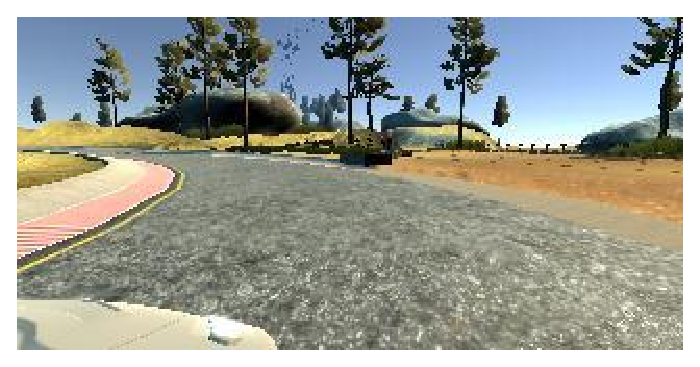
\includegraphics[width=0.98\linewidth]{figures/center_right.eps}
  \caption{Right camera}
\end{subfigure}
\label{fig:center_lane_driving}
\caption{Center lane driving}
\end{figure}

The training data with center lane driving only is of course not sufficient. There is always a situation when the neural network has to predict how to recover from the left or right sides of the road back to the center. I model this recovering by recording the vehicle driving on the left and right sides of the road applying the correction steering angles during the model training. The left, center and right cameras are taken into account. These images show what a left lane driving looks like:

\begin{figure}[H]
\centering
\begin{subfigure}{.3\textwidth}
  \centering
  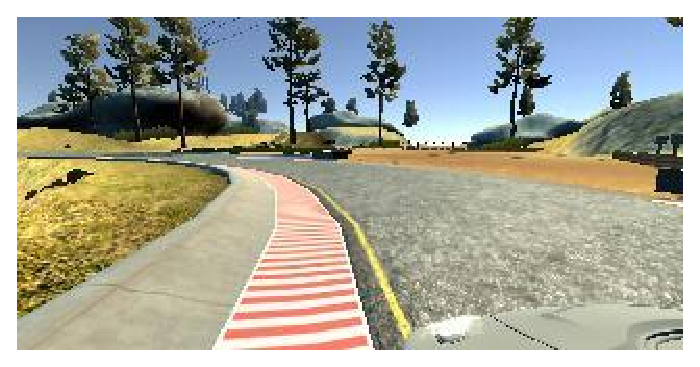
\includegraphics[width=0.98\linewidth]{figures/left_left.eps}
  \caption{Left camera}
\end{subfigure}
\begin{subfigure}{.3\textwidth}
  \centering
  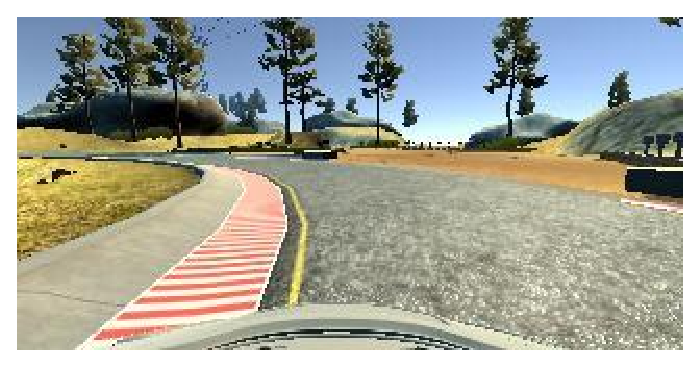
\includegraphics[width=0.98\linewidth]{figures/left_center.eps}
  \caption{Center camera}
\end{subfigure}
\begin{subfigure}{.3\textwidth}
  \centering
  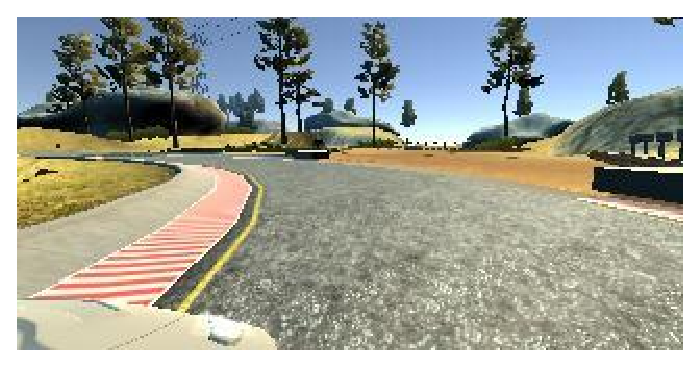
\includegraphics[width=0.98\linewidth]{figures/left_right.eps}
  \caption{Right camera}
\end{subfigure}
\label{fig:left_lane_driving}
\caption{Left lane driving}
\end{figure}

The right lane driving looks as follows:
\begin{figure}[H]
\centering
\begin{subfigure}{.3\textwidth}
  \centering
  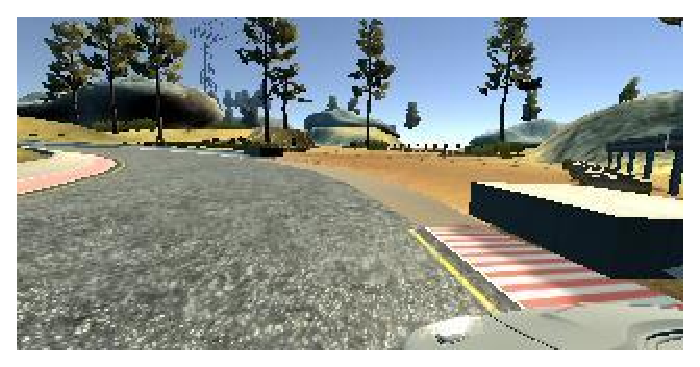
\includegraphics[width=0.98\linewidth]{figures/right_left.eps}
  \caption{Left camera}
\end{subfigure}
\begin{subfigure}{.3\textwidth}
  \centering
  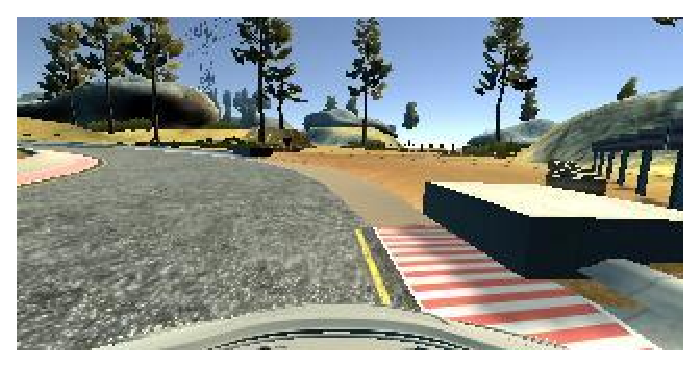
\includegraphics[width=0.98\linewidth]{figures/right_center.eps}
  \caption{Center camera}
\end{subfigure}
\begin{subfigure}{.3\textwidth}
  \centering
  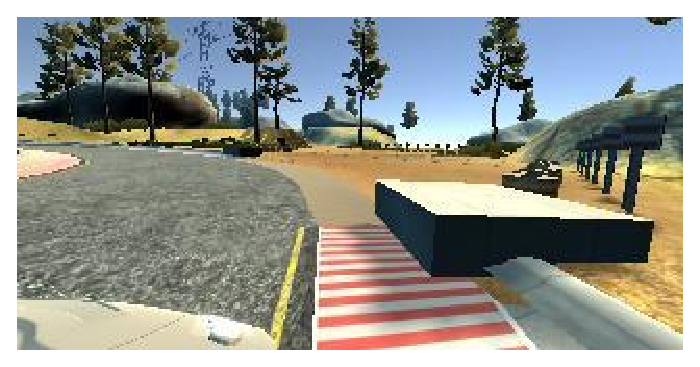
\includegraphics[width=0.98\linewidth]{figures/right_right.eps}
  \caption{Right camera}
\end{subfigure}
\label{fig:right_lane_driving}
\caption{Right lane driving}
\end{figure}
\noindent Therefore, the correction steering angles in left, center and right lane driving are as follows:
\begin{center}
  \begin{tabular}{| l | r | r | r |}
  \hline
   & Left Camera & Center Camera & Right Camera\\
    \hline
    Left Lane Driving & $+0.35$ & $+0.25$ & $+0.15$ \\ 
    Center Lane Driving & $+0.1$ & $0$ & $-0.1$ \\ 
    Right Lane Driving &  $-0.15$ & $-0.25$ & $-0.35$ \\
    \hline
  \end{tabular}
\end{center}
Therefore, the absolute value steering angle correction, $|\alpha|$, is proportional to the distance from the vehicle center to the center of the track, $l$:
$$
 \frac{d |\alpha|}{dl} > 0.
$$
\noindent This means that if the vehicle drives on the left side of the road, the algorithm sets the high absolute value of steering angle with the positive sign. If the vehicle drives on the right side of the road, the algorithm also sets the high absolute value of the steering angle but with the negative sign. In both cases the corrected steering angles bring the vehicle back to the lane center.

To augment the data set, I also flipped images and angles because this gives more data points.

After the collection process, I had 6267 data points of the center lane driving, 2904 -- of the left lane driving and 3168 -- of the right lane driving. I then preprocessed the images by normalizing it mapping values from 0 to 255 to the interval between $-0.5$ and $0.5$.

I finally randomly shuffled the data set and put 20\% of the data into a validation set. Other 80\% I used as training data for training the model. The validation set helped determine if the model was over or under fitting. The ideal number of epochs was 5 that provided already a low mean squared error. I used an Adam optimizer so that manually training the learning rate wasn't necessary.

\section{Simulation}
No tire leaves the drivable portion of the track surface. The car does not pop up onto ledges or roll over any surfaces that would otherwise be considered unsafe (if humans were in the vehicle).

\end{document}